\documentclass[11pt]{article}

\usepackage[utf8]{inputenc}
\usepackage[french]{babel}
\usepackage[rigidchapters]{titlesec}
\usepackage{comment,fullpage}
\usepackage{hyperref}
\usepackage{comment,times,fancyvrb,amsmath,amsthm,amssymb,latexsym,xspace}
\usepackage{graphicx}
\usepackage{palatino}

\usepackage{minted}

\graphicspath{{../figures/}}

% Palatino for rm and math | Helvetica for ss | Courier for tt
\usepackage{mathpazo} % math & rm
\linespread{1.05}        % Palatino needs more leading (space between lines)
\usepackage[scaled]{helvet} % ss
\usepackage{courier} % tt
\normalfont

\usepackage[T1]{fontenc}
\usepackage{color}
\usepackage{lastpage}
%\usepackage{verbatim}
%\usepackage{enumitem}
%\usepackage{moreverb}


%\setenumerate[0]{font=\itshape, label*=\thesection.\arabic*}


\newcommand{\guill}[1]{<<\,#1\,>>}




\begin{document}


\title{\textbf{ {}}}
\author{}
\date{\empty}

%\maketitle

%\tableofcontents

%\newpage
\thispagestyle{empty}

\begin{center}
\vspace*{1cm}
{\huge Projet ANR CollabScore}

\vspace{+1cm}

{\Large AAP Culture, créations, patrimoine \\
~\vspace*{0.2cm}
%Laboratoire \textsc{Cedric}\\
%~\vspace*{0.2cm}
%Conservatoire National des Arts et Métiers
}

\vspace{+1cm}
{\huge\bf Rapport intermédiaire (octobre 2022)}

\vspace{+1cm}

\end{center}


\begin{small}
\tableofcontents
\end{small}

\newpage

%%%%%

\section{Résumé du projet}

Les collections de partitions musicales constituent une part 
significative des fonds documentaires gérés par les bibliothèques patrimoniales. 
L’intégration de ces collections dans leurs bases de données est souvent déjà partiellement réalisée, 
mais elle se limite à la production d’images numériques (JPEG) que nous appelons \emph{partitions-images}. 
La nature particulière de la musique notée restreint considérablement les possibilités 
d’exploitation de telles sources. La simple recherche “plein texte” est par exemple impossible. 

Il est toutefois concevable de construire de telles méthodes d’interaction 
en se basant sur un codage structuré (XML) de la notation musicale, 
tel que le format  proposé par la Music 
Encoding Initiative [MEI]. La granularité très fine de ces représentations, que nous 
appelons \emph{partitions-notées}, permet d’en extraire des structures aptes 
à supporter des opérations de recherche, d’annotation et de mise en correspondance. 
Ces perspectives se heurtent cependant à un obstacle principal : la production de notation 
musicale numérique est notoirement difficile. Il n’existe à notre connaissance que trois 
méthodes : l’édition manuelle ; la transcription automatique d’une source audio ; 
la reconnaissance optique d’une partition existante (Optical Music Recognition, que nous francisons
en ``omérisation'' ci-dessous). 
Elles sont à l'heure actuelle 
soit très coûteuses (édition manuelle) soit très peu fiables (analyse audio et OMR). 

\subsection{Objectifs}

L’objectif du projet CollabScore est 
(i) de lever les obstacles à l’extraction à grande échelle du contenu des partitions-image, 
(ii) de décrire ce contenu avec le langage de la notation musicale, et enfin 
(iii) d’utiliser cette description comme support à la réalisation d’applications et d’interactions 
innovantes pour la valorisation des fonds musicaux.

 
Le projet est structuré autour de trois objectifs complémentaires:
\begin{enumerate}

  \item Conception, mise en place et validation d’un \emph{processus collaboratif} de numérisation du contenu 
      prenant des partitions-images en entrée et produisant des partitions-notées.
  \item Utilisation de cette notation comme pivot pour l’association fine de sources multimodales, 
     images, audios ou vidéos, grâce à un \emph{alignement} au niveau de la mesure.
   \item Enfin, \emph{démonstration} du potentiel de cette notation comme support à des dispositifs d’interaction et 
     d’enrichissement, soit à destination du grand public (écoute en ligne, pédagogie, pratique personnelle), 
      soit pour des experts musiciens et musicologues (analyse comparative des sources).
\end{enumerate}

La première action implique une démarche de recherche pluridisciplinaire visant à lever plusieurs verrous : 
amélioration des résultats de l’OMR via des techniques d’apprentissage ; détection automatique des anomalies ; 
amélioration d’une partition-notée via un environnement collaboratif.  La seconde s’appuie sur des méthodes de 
mise en correspondance de la partition notée avec d’autres sources multimodales, 
correspondance nommée ``alignement'' dans ce document. 
La dernière action mettra en place chez deux des partenaires du projet, représentatifs d’institutions en 
charge de fonds musicaux patrimoniaux, des démonstrateurs s’appuyant sur les partitions-notées.  

\subsection{Structure du projet}

La figure~\ref{schema-projet} résume l'organisation du projet CollabScore.
Les phases 1 et 2 du projet prennent en entrée une partition-image, 
soit typiquement les scans des fonds musicaux tels qu’on peut les trouver 
sur Gallica, et en extraient une description du contenu sous forme de notation musicale. 
Le codage de ce contenu, la partition-notée, s’appuiera sur le format MEI, 
plus adapté que MusicXML aux tâches de philologie numérique. Ce format
 est maîtrisé par les partenaires qui l’utilisent depuis des années. 
 
  \begin{figure}[htb]
  \begin{center}
   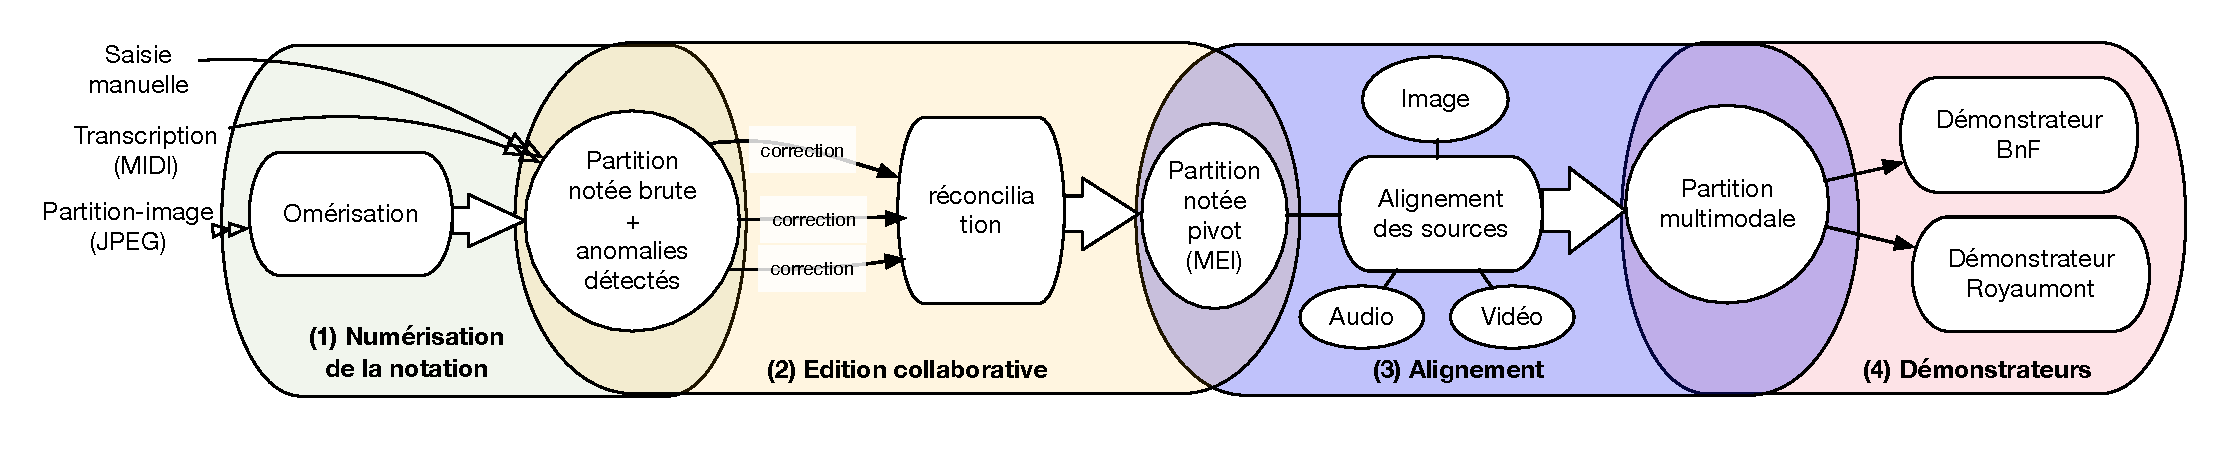
\includegraphics[width=\textwidth]{schema_projet.pdf}
    \caption{Schéma du projet}
    \label{schema-projet}
    \end{center}
  \end{figure}

 
 La phase 3 utilise la partition-notée comme pivot pour lier plusieurs sources 
 multimédia relatives au même contenu (image, texte, audio, vidéo…). 
 Enfin la quatrième phase consiste à produire des démonstrateurs  
 chez les partenaires-utilisateurs du projet sur la base des méthodes, outils et formats précédents.

\subsection{Consortium}

Le project est coordonné par Philippe Rigaux, Professeur des Universités au Cnam. Il comprend les partenaires suivants\,:

\begin{itemize}
  \item Le Cnam intervient dans le projet d’une part en recherche sur les méthodologies de \textit{crowdsourcing} 
    (plate-forme en collaboration avec la BnF), et d’autre part comme maître d’œuvre pour la réalisation des démonstrateurs.
  \item La BnF prend la responsabilité de l’environnement de crowdsourcing, en lien avec le Cnam (Lot 2). 
    Elle assurera la communication auprès des communautés ciblées, le recrutement des volontaires, 
    le suivi et l’animation de la campagne, l’évaluation des résultats. 
    
   \item L’IReMus collabore avec l’IRISA sur les aspects méthodologiques et musicologiques de la numérisation.
     \item L'IRISA  concentrera ses travaux sur la fiabilisation de l’omérisation des partitions et l’identification 
       des fragments défaillants en sortie, en association avec l’IReMus pour les aspects musicologiques (syntaxe de la notation).
  \item
  La Fondation Royaumont interviendra comme utilisateur et validateur du démonstrateur final : mise à disposition des partitions-image et autres sources (audio), contrôle des numérisations, diffusion auprès de la communauté des bibliothèques musicales. 
 \item Le laboratoire CRIStAL (Univ. Lille, équipe AlgoMus)  contribue
    au développement de la  plateforme, pour tout ce qui concerne l'édition et
  l'affichage de sources synchronisées à une partition-pivot.
\end{itemize}

Il est important de noter que le consortium a évolué par l'intégration comme partenaire
de l’équipe d'informatique musicale Algomus de l’Université de Lille (laboratoire
CRIStAL). Algomus  développe depuis plusieurs années Dezrann, une plateforme libre pour écouter, étudier et annoter
la musique sur le web, utilisée pour la recherche et la pédagogie. Après échanges
avec le Cnam, il est apparu que CollabScore et Dezrann
partagent des concepts similaires, notamment la notion de partition-pivot, la
référence étant le temps musical, et la considération de sources annexes.
Algomus a par ailleurs déjà développé des interfaces comparables à celles
envisagées pour le projet CollabScore et dispose des compétences pour réaliser une
partie bien identifiée des tâches du projet initialement allouées au Cnam. L’Université de Lille 
a donc rejoint en juin 2022, soit plus d'un an après le début de la période scientifique, 
le projet ANR CollabScore pour contribuer
au développement de la nouvelle plateforme, pour tout ce qui concerne l'édition et
l'affichage de sources synchronisées à une partition-pivot.

\subsection{Planification initiale des tâches}

Le plan initial du projet a été décrit en détail dans le document de soumission.
La figure~\ref{gantt} en donne un résumé sous la forme d'un diagramme de Gantt. Nous
faisons référence à ce plan par la suite pour évaluer l'avancement du projet. 


  \begin{figure}[htb]
  \begin{center}
   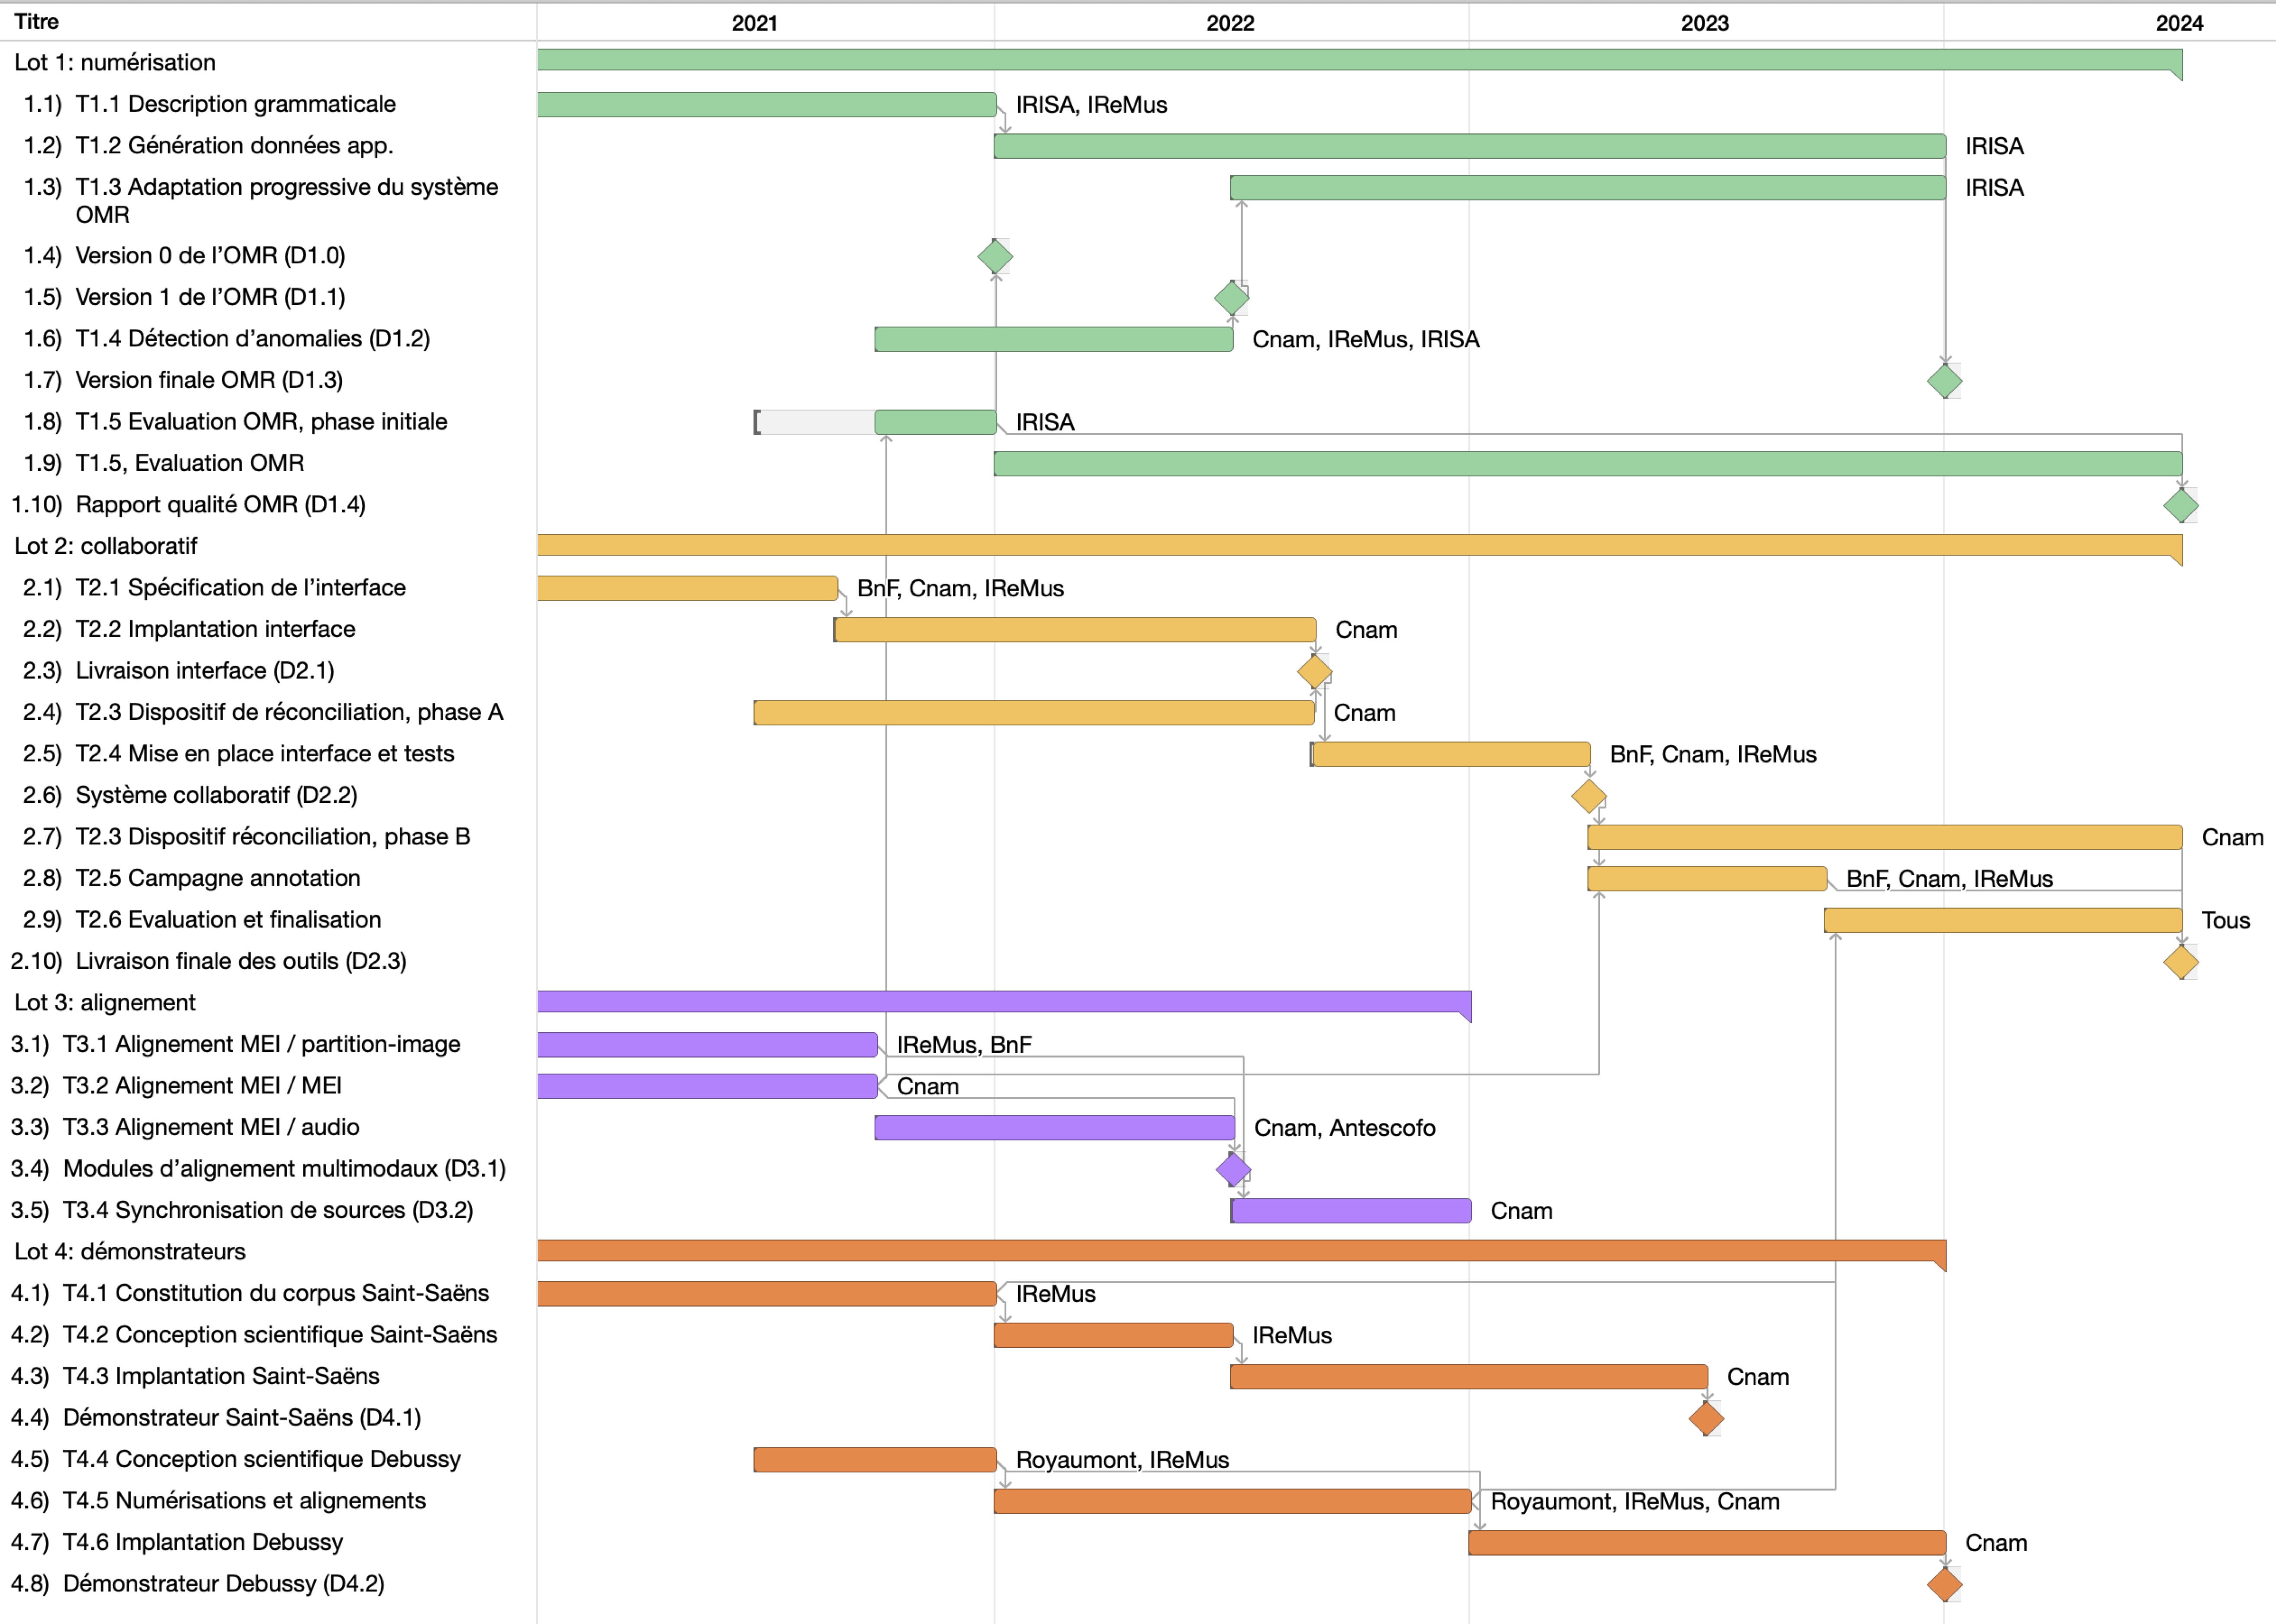
\includegraphics[width=\textwidth]{gantt}
    \caption{Diagramme décrivant la planification du projet}
    \label{gantt}
    \end{center}
  \end{figure}
  
\section{Travaux effectués durant la première phase du projet}

La période scienfifique du projet s'étend d'avril 2021 à juin 2024 (42 mois). En raison de plusieurs
événements ayant partiellement affecté les premières phases du projet (restrictions Covid, difficultés de 
recrutements et délai administratif d'intégration du nouveau partenaire), nous souhaitons 
prolonger de 6 mois cette période. Nous y revenons dans la section consacrée au bilan, 
page~\pageref{sec:bilan}, 

\subsection{Lot 0\,: coordination}

Ce lot est sous la responsabilité du Cnam. Le coordinateur a mis en place un ensemble d'outils permettant 
la communication autour du projet, l'intégration et le suivi de l'ensemble des lots. Ces outils sont
centrés sur un dépôt Github (\url{https://github.com/collabscore})
qui rassemble les modules informatiques partagés par les partenaires, les jeux de données 
ainsi que la documentation du projet.

Le Cnam a consacré l'essentiel de ses ressources à la mise en place d'un serveur \emph{CollabScore} constitué

\begin{enumerate}
 \item d'un dépôt de partitions multimodales consultables à l'adresse \url{http://neuma.huma-num.fr/home/corpus/collabscore/}\,;
  \item  de fonctionnalités internes développées par le Cnam visant notament à permettre la réconciliation 
       de corrections collaboratives ; ces fonctionnalités sont accessibles aux partehaires dans un espace privé\,;
   \item  d'une interface Web pour les interactions utilisateurs (en cours de développement, version
         préliminaire consultable par exemple ici \url{http://neuma.huma-num.fr/home/opus/collabscore:dmos_ex1/})\,; 
  \item et d'une interface de services REST pour les communications avec tous les modules développés par les autres 
      partenaires du projet.
\end{enumerate}

  \begin{figure}[htb]
  \begin{center}
   \includegraphics[width=12cm]{architecture.pdf}
    \caption{Architecture technique}
    \label{architecture}
    \end{center}
  \end{figure}
  
L'architecture à base de services est résumée dans la figure~\ref{architecture}.
Elle est conçue pour permettre à chaque partenaire de développer ses outils indépendamment, 
la seule contrainte technique étant
d'établir un canal de communication avec le serveur CollabScore via ses services.  

Le serveur est en place. Une partie des services REST, principalement ceux permettant 
de récupérer les fichiers constituant une partition multimodale, et de déposer des annotations, a 
été développée et mise à disposition des partenaires impliqués dans les développements informatiques.


\subsection{Lot 1\,: reconnaissance optique (omérisation)}

Le module OMR est à peu près entièrement à la charge de l'IRISA. Le principe de l'intégration au reste de 
l'architecture est le suivant: le module OMR (DMOS) interroge le serveur CollabScore pour obtenir des partitions multimodales.
Pour chacune, la source originale peut être récupérée par URL, traitée par l'OMR, avec production d'une partition
pivot (document MEI) et des annotations indiquant les parties à confirmer ou contrôler. 
DMOS transmet via un appel REST l'ensemble de ces informations sous la forme d'un document JSON 
qui est ingéré par le serveur CollabScore et converti en MEI.

Contrairement à ce qui était envisagé, le module OMR n'a pas pu être utilisé
rapidement, même dans une version très simplifiée,  à cause de problèmes de recrutement. 
Depuis septembre 2022, 
l'ensemble de la chaîne de transformation est  fonctionnel et permet de traiter
des cas simples de numérisation. Les prochaines étapes consistent à augmenter progressivement le
niveau des difficultés traitées, en fonction d'une liste d'œuvres de référence établie par l'IRéMus.
La situation à ce jour correspond à l'état attendu à T0+12 (tâche T1.1) 
soit un retard de 6 mois.

\subsection{Lot 2\,: collaboratif}

Ce lot a pris du retard en raison, d'une part, des difficultés initiales rencontrées par le projet 
et, d'autre part, d'une dépendance 
sous-estimée au départ avec le lot 1 (omérisation) dont dépend la mise à disposition de données.
La conception d'une interface de correction collaborative est
en effet fonction des types d'erreur rencontrées et remontées par l'OMR, et le décalage dans la
mise en œuvre de ce dernier s'est donc reporté sur le Lot 2. Nous 
sommes, à ce jour, en mesure de commencer l'étude de l'interface initialement prévue à T0.
Ce retard n'est pas si impactant que sa durée apparente de 18 mois pourrait le suggérer. 
Le Cnam est en effet déchargé de la responsabilité des lots d'alignement (pris en charge par Algomus)
et va pouvoir se concentrer sur les aspects collaboratifs. De plus, la dépendance mentionnée ci-dessus
aurait, dans tous les cas, induit nécessairement un décalage sur la date de début de cette étude.


\subsection{Lot 3\,: alignement}

Les tâches d'alignement ont pour l'essentiel (tâches T3.1, T3.3 et T3.4) été transférées au nouveau partenaire Algomus. 
La date d'entrée de ce partenaire étant à T0+15, on peut considérer en première approche que
les tâches T.1 et T3.3 seraient décalées d'autant. En fait, les compétences de ce nouveau partenaire 
couvrant déjà en  partie les fonctionnalités attendues, la réalisation de ces tâches
s'effectuera à court terme. En particulier, l'alignement partition pivot-audio (tâche T3.3) est toujours
prévue fin 2022, soit dans les délais planifiés initialement. La tâche T3.1 
(alignement partition pivot-image) interviendra dans le premier semestre 2023, avec un 
retard estimé à une année.

\subsection{Lot 4\,: démonstrateurs}

Ce lot est le dernier à intervenir  (temporellement) dans le projet car sa réalisation 
dépend de l'ensemble des modules développés dans les autres lots. La constitution du corpus 
qui servira au premier démonstrateur (œuvres de Saint-Saens, tâche T4.1) est en cours de constitution
par l'IRémus et déjà bien avancée, avec notamment les liens vers les partitions-image
des ces œuvres disponibles sur Gallica. 

\section{Bilan, réorganisations et extension}\label{sec:bilan}

À l'issue de ce bilan rapide, nous considérons que le projet est sur de bons rails
et que les objectifs initiaux peuvent être confirmés. Leur 
durée de réalisation, ainsi que le séquencement des différentes tâches, doivent 
cependant être révisé, \textbf{par une extension de 6 mois de
la période scientifique}. 

\subsection{Difficultés du projet}

Le projet a rencontré des difficultés initiales sur lesquelles nous revenons
pour les synthétiser.
 
\begin{enumerate}
  \item Les restrictions liées ont covid ont eu un réel impact puisque le dernier confinement 
     est intervenu en avril 2021, quelques jours après le début théorique du projet. Même 
     si les restrictions ont cessé fin juin  2021, les six premiers mois ont été fortement
     affectés, et l'ensemble de cette période tourmentée a induit une remise en route laborieuse
     de nos modes de travail, peu propice en tout cas à un travail collaboratif.
    \item Nous avons rencontré de fortes difficultés de recrutement. En particulier, l'IRISA
     a attendu longtemps avant de trouver de bons candidats, et a choisi de diviser le travail
      en deux, les deux ingénieurs recrutés débutant pendant l'été 2022. Cette division doit permettre
      de rattraper -- mais seulement en partie -- le retard par la mise en parallèle des tâches. Ces difficultés
      ont également affecté le Cnam qui souhaitait initialement recruter un doctorant et s'est finalement
      tourné vers un post-doctorant concentré sur les tâches de \textit{crowdsourcing}, après
      délégation des tâches d'alignement à Algomus.
    \item Enfin, l'introduction d'un nouveau partenaire a entrainé des délais administratifs importants.    
\end{enumerate}


\subsection{Mesures de réorganisation}

Les obstacles mentionnés précédemment ont entraîné un
retard de mise en œuvre que l'on pourrait estimer à une année. Nous avons cependant compensé
en partie ce retard par quelques changements, consistant  essentiellement en une parallélisation
des tâches. L'IRISA emploie deux ingénieurs sur 18 mois, au lieu d'un sur 36 mois comme envisagé 
au départ. Le Cnam a confié une partie des tâches du lot 3 au nouveau partenaire, Algomus, 
ce qui permet là encore de travailler en parallèle sur les tâches collaboratives d'une part, et
d'alignement d'autre part.  Là encore, ce partage doit permettre d'effectuer les travaux envisagés
avec décalage, mais dans les limites de temps du projet.

Le principal impact concerne le Lot 2, consacré aux opérations de correction collaborative. En raison
de leur dépendance vis-à-vis de l'omérisation et du décalage de cette dernière, nous devons envisager 
une réorganisation consistant à décaler de 6 mois la période de travail pour les tâches du Lot 2,
ainsi que la réalisation des démonstrateurs du Lot 4.

\subsection{Demande d'extension}

En résumé, le projet CollabScore est maintenant pleinement dans sa phase de réalisation, 
et nous confirmons les objectifs visés initialement. Nous demandons 
cependant à l'ANR une extension de 6 mois de la période de travail scientifique afin
de compenser les décalages dus aux difficultés de début de projet.
 
\end{document}